\subsubsection{Figure et démonstration}

Les exercices de géométrie occupent une place centrale dans les compétitions de mathématiques. Quand vous voyez un exercice de géométrie, le premier réflexe est de faire une figure. Prenez l'habitude de les faire en utilisant une règle, une équerre et un compas. C'est le matériel autorisé aux compétitions internationales. Ceci dit, une figure seule ne suffit pas à résoudre un exercice de géométrie, elle permet seulement de le vérifier dans un cas particulier, à condition qu'elle soit faite suffisament soigneusement (notez bien que plus une figure est grande, plus il est facile de la faire soigneusement, plus on arrive à voir ce qui se passe). Illustrons ceci avec un résultat classique.

\begin{thm}
Dans un triangle, la somme des angles vaut $180^\circ$.
\end{thm}

Vous pouvez évidemment faire une figure soigneusement et vérifier à l'aide d'un rapporteur (par ailleurs interdit à la plupart des compétitions de mathématiques) que la somme des angles vaut $180^\circ$. Ceci dit, comment en être sûr que c'est vrai quelque soit le triangle que vous tracez ? Il faut en faire la démonstration ! Ceci dit, il est illusoire de faire une démonstration sans faire de figure. C'est pourquoi dans les entraînements d'Animath, on vous accorde 1 point (sur 7) pour un exercice de géométrie où vous avez fait une figure correctement. Il s'agit de la première étape dans la résolution d'un exercice. La figure peut aussi vous permettre de comprendre comment faire la démonstration.

\begin{preuve}
Traçons un triangle $ABC$, dont on notera les angles $\alpha,\beta,\gamma$ (il s'agit d'une notation habituelle).
\centering{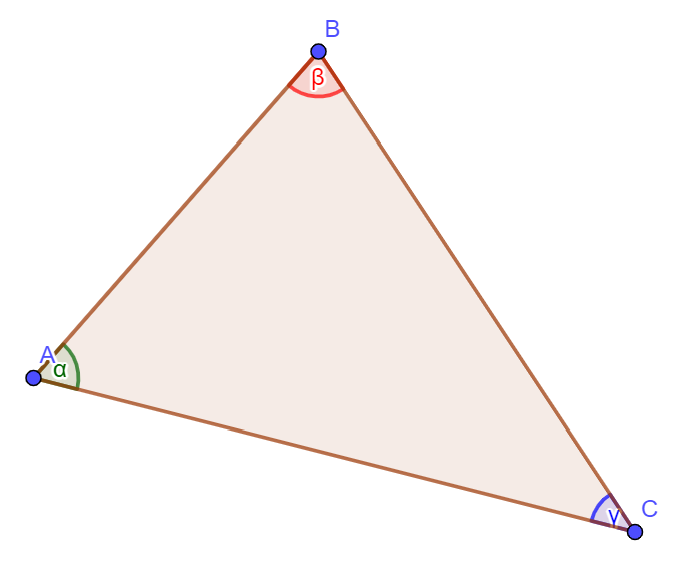
\includegraphics[scale=1]{A-17-PM/A-17-PM-0.png}}\newline
On trace la droite parallèle passant par $A$ et parallèle à $(BC)$, ce qui nous permet de noter des égalités d'angles, d'après l'égalité des angles alternes-internes.
\centering{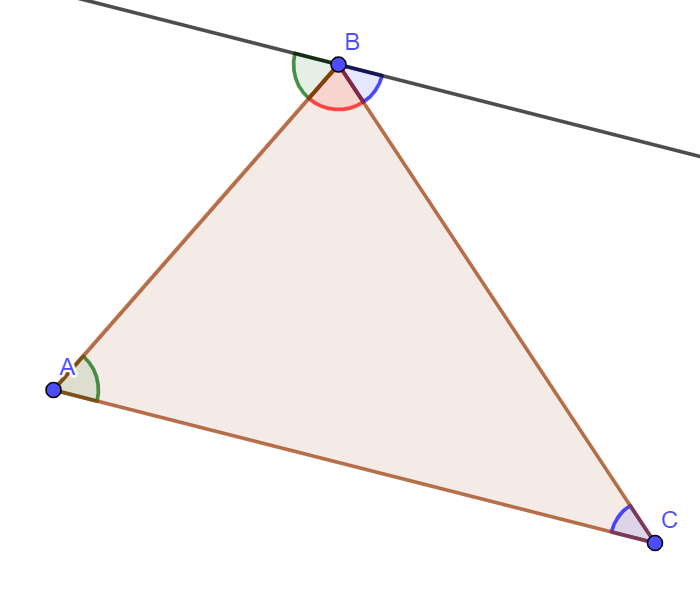
\includegraphics[scale=1]{A-17-PM/A-17-PM-1.png}}\newline
Ceci nous démontre que $\alpha+\beta+\gamma$ correspond à l'angle plat, i.e. $180^\circ$.
\end{preuve}

Notons que ce résultat peut être généralisé pour un polygone à $n$ côtés. Nous allons nous limiter aux polygones convexes ici (pour ceux qui ne savent pas ce que c'est, vous allez bientôt l'apprendre !), mais ce résultat est aussi valide pour les polygones non convexes.

\begin{thm}
La somme des angles d'un polygone (convexe) à $n$ côtés vaut $180^\circ(n-2)$.

En particulier, la somme des angles d'un quadrilatère vaut $360^\circ$.
\end{thm}

\begin{preuve}
Remarquons tout d'abord qu'un quadrilatère peut être décomposé en deux triangles en traçant une diagonale.
\centering{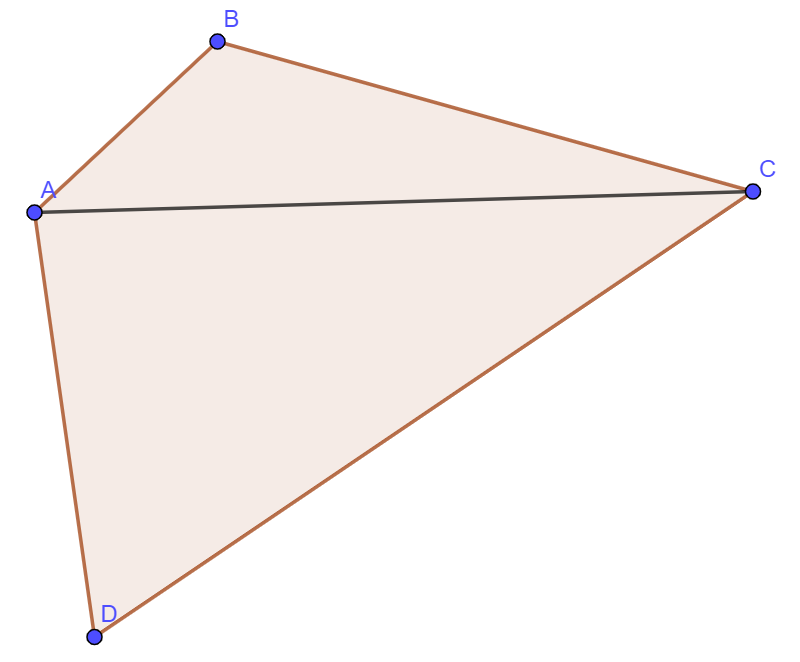
\includegraphics[scale=1]{A-17-PM/A-17-PM-2.png}}\newline
Ainsi, la somme des angles du quadrilatère vaut la somme des des angles des deux triangles, donc $2 \dot 180^\circ$, i.e. $360^\circ$.

Pour le cas général, on peut imaginer deux approches. La première consiste à supposer que vous avez déjà démontré le théorème pour un polygone à $n$ côtés (par exemple, $n=4$ car on a effectivement déjà démontré que la somme des angles d'un quadrilatère vaut $180^\circ \cdot (4-2)$), et de démontrer ce théorème pour un polygone à $n+1$ côtés. Prenons un polygone à $n+1$ côtés $ABCDE...$ et traçons la diagonale $AC$ comme sur la figure :
\centering{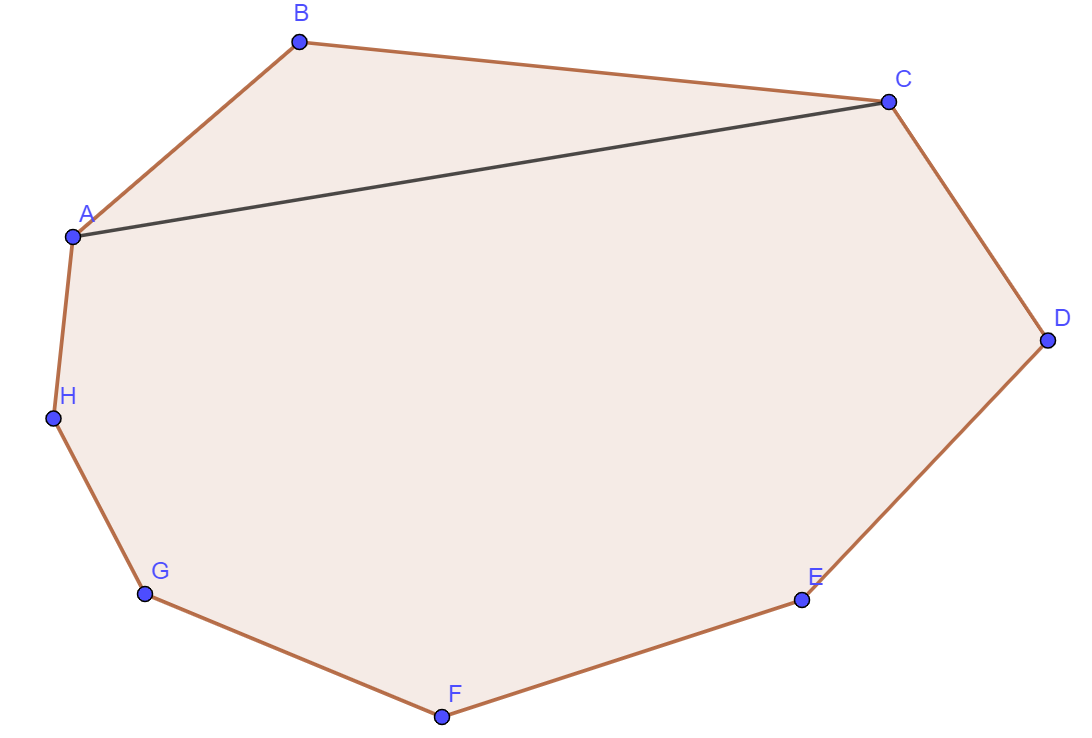
\includegraphics[scale=1]{A-17-PM/A-17-PM-3.png}}\newline
Ainsi, le polygone à $n+1$ côtés est partagé en un triangle $ABC$ et un polygone à $n$ côtés $ACDE...$. Donc, la somme des angles du polygone à $n+1$ côtés vaut la somme des angles d'un triangle auquel on rajoute la somme des angles d'un polygone à $n$ côtés, i.e. $180^\circ+180^\circ\cdot(n-2)=180^\circ\cdot((n+1)-2)$. Ainsi, après avoir démontré ce théorème pour un quadrilatère, vous le démontrez pour un pentagone, puis pour un hexagone, puis pour un heptagone, puis pour un octogone, etc. Vous verrez plus tard que ce genre de raisonnement s'appelle un raisonnement par récurrence.

La deuxième approche consiste à prendre un point $O$ à l'intérieur du polygone et le joindre à tous les sommets du polygone par des segments.
\centering{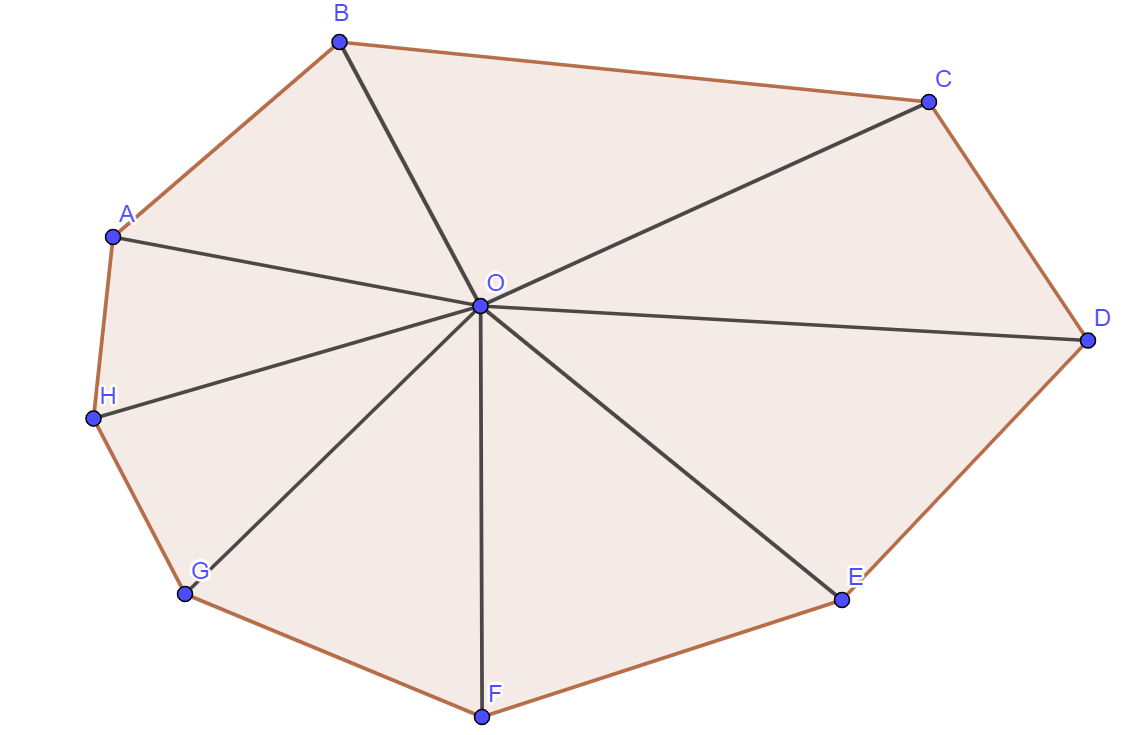
\includegraphics[scale=1]{A-17-PM/A-17-PM-4.png}}\newline
Ainsi, on voit apparaître $n$ polygones. On observe que si on somme les angles de tous les triangles, on obtient la somme des angles du polygone auquel il faut rajouter la somme de tous les angles autour de $O$. La somme des angles de tous les triangles vaut $180^\circ\cdot n$ car il y a $n$ triangles. La somme des angles du polygone est ce qu'on cherche. Et la somme de tous les angles autour de $O$ vaut $360^\circ$ (l'angle plein).

Ainsi, la somme des angles d'un polygone à $n$ côtés vaut
\[
180^\circ \cdot n - 360^\circ = 180^\circ\cdot(n-2).
\]
\end{preuve}

\subsubsection{Quelques révisions sur les triangles égaux}
Nous vous renvoyons à votre cours de collège pour l'énoncé des trois cas d'égalité des triangles. Rappelons que quand on parle des triangles égaux, il est important de faire attention à l'ordre dans lequel on écrit les sommets (si un triangle $ABC$ est égal à un triangle $DEF$, il n'est pas forcément égal au triangle $EDF$). C'est un des premiers outils dont il faut savoir se servir pour les exercices. Pour trouver ce qu'il faut démontrer dans les deux exercices suivants, il faut commencer par faire une belle figure et émettre des conjectures.

\begin{exo}
Soit $ABC$ un triangle avec $AB=AC>BC$. Soit $E$ sur la droite
$(AB)$ qui soit à l'extérieur du triangle $ABC$ tel que $BE=AB-BC$. Soit
$D$ sur la droite $(BC)$ qui soit à l'extérieur du triangle $ABC$ du côté
de $C$ tel que $CD=AB-BC$. Que dire du triangle $ADE$ ?
\end{exo}

\begin{sol}
On commence par faire une jolie figure et on fait des mesures sur la figure pour faire des conjectures.
\centering{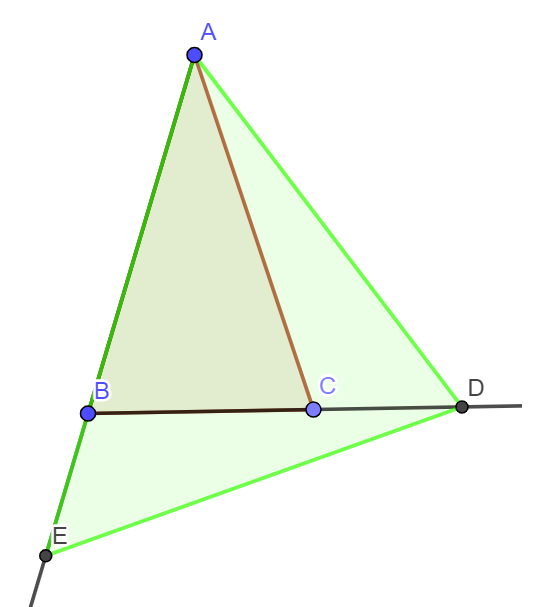
\includegraphics[scale=1]{A-17-PM/A-17-PM-5.png}}\newline
Vous avez probablement remarqué que le triangle $ADE$ est isocèle en $D$, mais n'est pas équilatéral, ni rectangle.

Essayons maintenant de le démontrer. On veut montrer que $ED=DA$. En observant la figure, on est tenté de montrer que le triangle $BED$ est égal au triangle $CDA$, ce qui implique l'égalité des longueurs voulue. Pour y arrivons, utilisons le premier cas d'égalité des triangles et montrons que $BE=CD$, $BD=CA$ et $\widehat{EBD}=\widehat{DCA}$. Tout d'abord, $BD=CD=AB-BC$ d'après l'énoncé. Puis, $BD=BC+CD=BC+(AB-BC)=AB=CA$ d'après l'énoncé. Enfin, $\widehat{EBD}$ est supplémentaire à $\widehat{ABC}$, et $\widehat{DCA}$ est supplémentaire à $\widehat{ACB}$. Donc, comme $\widehat{ABC}=\widehat{ACB}$ d'après le critère du triangle isocèle, on a $\widehat{EBD}=\widehat{DCA}$.

Pour être exhaustif, on peut montrer que $ADE$ n'est ni équilatéral ni rectangle. Il n'est pas équilatéral car $DA<AC+CD$ d'après l'inégalité triangulaire (le chemin le plus court entre deux points est toujours la ligne droite), et $AC+CD=AB+BE=AE$ d'après les égalités des longueurs données par l'énoncé. Ainsi, $DA<AE$, donc $ADE$ ne peut être équilatéral.

Montrons que $ADE$ n'est pas isocèle rectangle en $D$ (juste isocèle mais pas rectangle). Pour cela, montrons que l'angle $\widehat{ADE}$ ne peut être droit. Observons que $\widehat{ADE}=\widehat{ADC}+\widehat{BDE}$. Enfin, comme le triangle $BED$ est égal au triangle $CDA$, on a que $\widehat{BDE}=\widehat{CAD}$. Ainsi, $\widehat{ADE}=\widehat{ADC}+\widehat{CAD}=180^\circ-\widehat{ACD}$ d'après la somme des angles dans le triangle $ACD$. Enfin, $\widehat{ACD}$ est supplémentaire à $\widehat{ACB}$, donc, $\widehat{ADE}=\widehat{ACB}$. Le dernier angle est aigu car c'est un angle de la base d'un triangle isocèle.
\end{sol}

\begin{exo}
Soit $ABCD$ un parallélogramme. On construit à l'extérieur de $ABCD$
des triangles équilatéraux $ADP$ et $ABQ$. Que dire du triangle
$PQC$ ?
\end{exo}

\begin{sol}
Comme d'habitude, on commence par une jolie figure et on fait des conjectures.
\centering{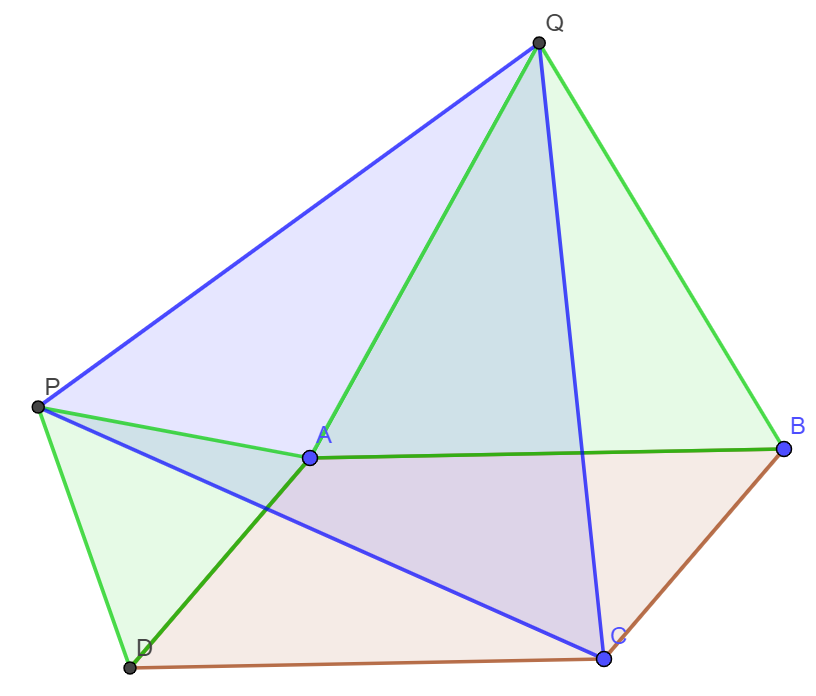
\includegraphics[scale=1]{A-17-PM/A-17-PM-6.png}}\newline
En voyant la figure, on conjecture que $PQC$ est équilatéral. Pour montrer que $QC=CP=QP$, la figure nous suggère de montrer l'égalité entre trois triangles. On va montrer que le triangle $QCB$ est égal au triangle $CPD$ et qui est lui-même égal au triangle $QPA$. Pour y arriver, nous allons utiliser le premier cas d'égalité, i.e. il suffit de montrer que $QB=CD=QA$, $CB=PD=PA$ et $\widehat{QBC}=\widehat{CDP}=\widehat{QAP}$. Pour la première égalité, $QB=AB$ et $QB=QA$ car $QAB$ est équilatéral, puis $AB=CD$ car $ABCD$ est un parallélogramme. Pour la deuxième égalité, $CB=AD$ car $ABCD$ est un parallélogramme, puis $AD=PD$ et $AD=PA$ car $APD$ est équilatéral. Pour la dernière égalité (celle à propos des angles), notons $\beta=\widehat{ABC}$, alors $\widehat{ADC}=\beta$ et $\widehat{DAB}=180^\circ-\beta$ d'après les égalités d'angles obtenues avec les droites parallèles. Ainsi, $\widehat{QBC}=60^\circ+\beta$ (d'après les angles du triangle équilatéral), $\widehat{CDP}=60^\circ+\beta$ également, et $\widehat{QAP}=360^\circ-2\cdot 60^\circ-(180^\circ-\beta)=60^\circ+\beta$. Ce qui conclut.
\end{sol}

\subsubsection{Introduction à la chasse aux angles}
Quand vous avez un exercice de géométrie devant vous, un des premiers réflexes est d'observer tous les angles qui sont présents sur la figure et de voir lesquels d'entre eux sont égaux. En pratique, on commence par noter un angle sur la figure à l'aide d'un petit arc de cercle et vous notez tous les angles égaux à celui-ci sur la figure avec le même arc de cercle grâce aux outils que vous avez pour déterminer que deux angles sont égaux. Puis, vous changez de couleur et notez un angle qui n'est pas égal au premier ainsi que tous les angles égaux à celui-ci. Et vous continuez !

Les outils dont vous disposez pour démontrer des égalités d'angles sont résumés à la fin du résumé de cette séance et nous avons surtout appris un nouvel outil : le théorème de l'angle inscrit.


\begin{dfn}
Soit $\mathcal{C}$ un cercle de centre $O$. On prend $A,B,C$ trois points sur $\mathcal{C}$. On dit que $\widehat{BAC}$ est un angle inscrit dans le cercle $\mathcal{C}$ qui intersepte l'arc $\stackrel \frown{BC}$ qui se trouve à l'intérieur de l'angle $\widehat{BAC}$ considéré. On dit que $\widehat{BOC}$ est l'angle au centre dans le cercle $\mathcal{C}$ qui intersepte l'arc $\stackrel \frown{BC}$ qui se trouve à l'intérieur de l'angle $\widehat{BOC}$.
\end{dfn}

Voici une figure qui permet d'illustrer le concept. Observez qu'il existe deux arcs de cercle qu'on peut nommer $\stackrel \frown{BC}$, ainsi que deux angles qu'on peut nommer $\widehat{BAC}$ ou $\widehat{BOC}$, mais la correspondance entre l'arc de cercle et l'angle inscrit est sans ambiguité. De plus, il y a une correspondance entre chaque arc de cercle et chaque angle au centre.
\centering{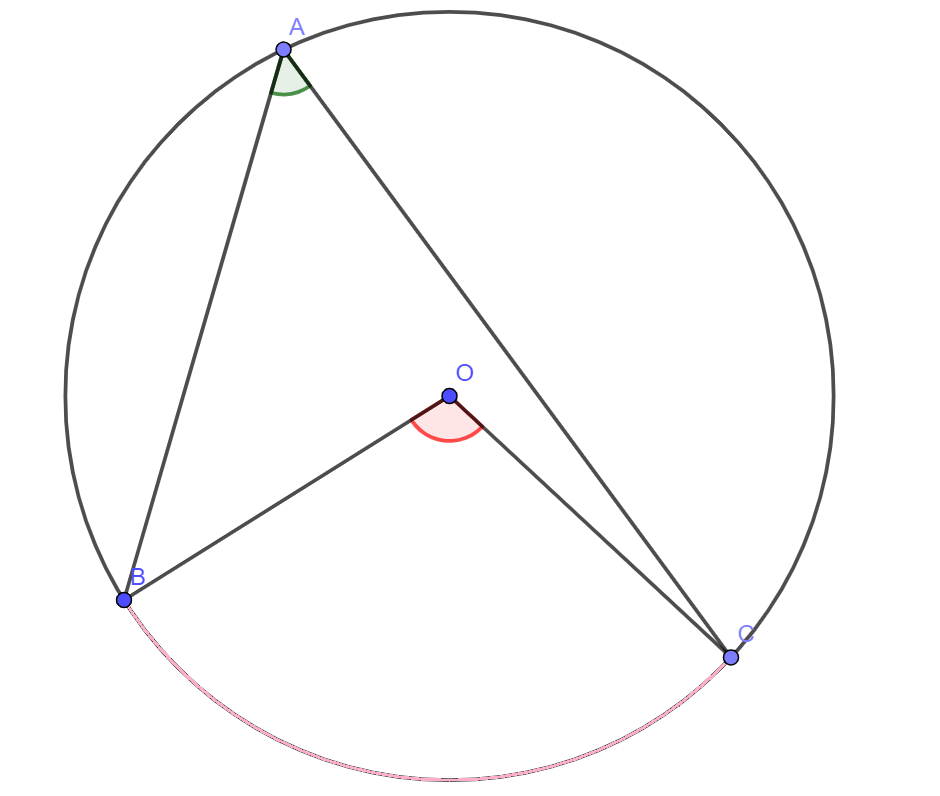
\includegraphics[scale=1]{A-17-PM/A-17-PM-7.png}}\newline

Voici le théorème de base dont nous avons besoin. C'est le théorème de l'angle au centre et de l'angle inscrit.

\begin{thm}
Soit $\mathcal{C}$ un cercle de centre $O$. On prend $A,B,C$ trois points sur $\mathcal{C}$. Soit $\widehat{BAC}$ un angle inscrit interseptant l'arc $\stackrel \frown{BC}$ et $\widehat{BOC}$ l'angle au centre associé. Alors,
\[
2\widehat{BAC}=\widehat{BOC}.
\]
\end{thm}

\begin{preuve}
Pour démontrer ce théorème, il convient de distinguer trois cas.

\underline{\textit{Premier cas :}} le cas où $O$ se trouve sur un côté de l'angle $\widehat{BAC}$.
\centering{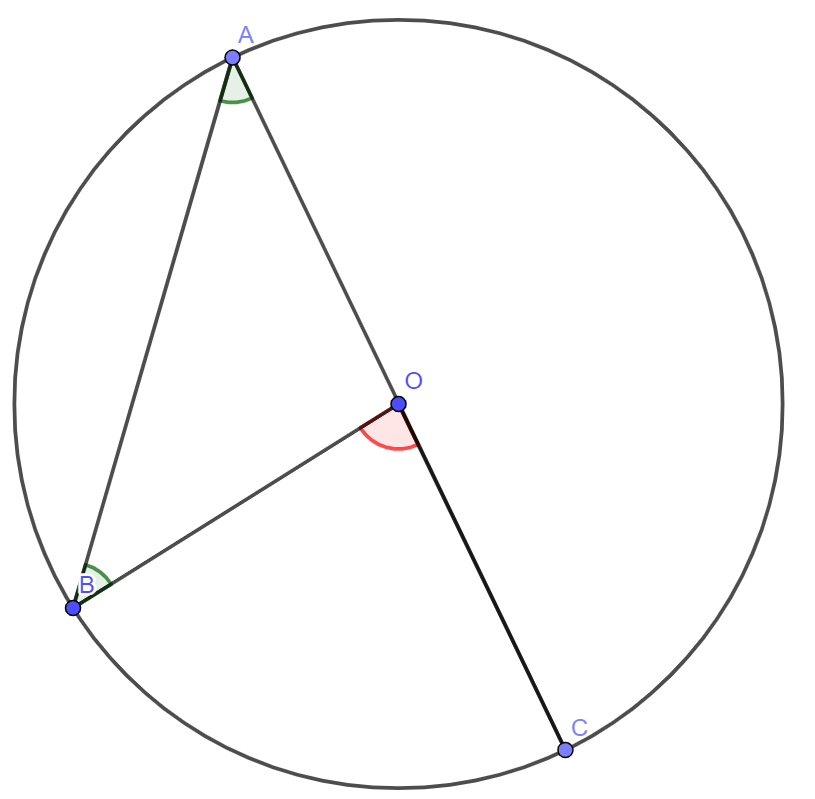
\includegraphics[scale=1]{A-17-PM/A-17-PM-8.png}}\newline
$\widehat{BOC}$ est supplémentaire à $\widehat{AOB}$, qui est lui-même supplémentaire à $\widehat{OAB}+\widehat{OBA}$ (d'après la somme des angles dans le triangle $OAB$). Comme le triangle $OAB$ est isocèle en $O$ ($OA=OB$ car c'est des rayons), on a $\widehat{OAB}=\widehat{OBA}$. Donc, $\widehat{BOC}=2\widehat{BAC}$.

\underline{\textit{Deuxième cas :}} le cas où $O$ se trouve à l'intérieur de l'angle $\widehat{BAC}$.
\centering{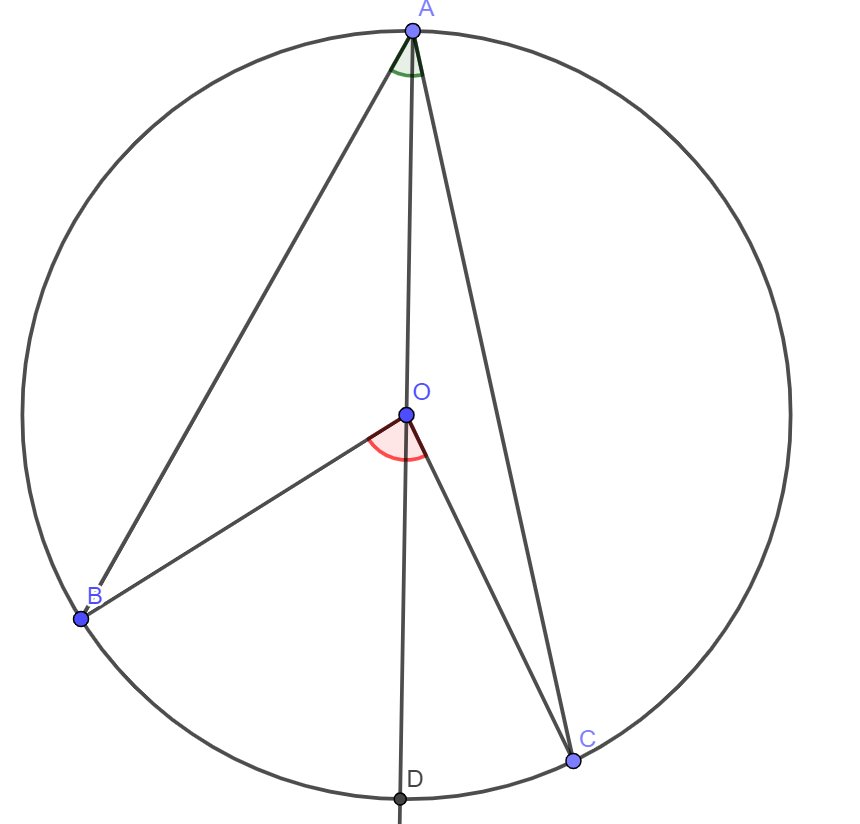
\includegraphics[scale=1]{A-17-PM/A-17-PM-9.png}}\newline
On trace le diamètre $AD$. Ceci partage l'angle $\widehat{BAC}$ en deux angles : $\widehat{BAD}$ et $\widehat{DAC}$. On utilise le premier cas pour affirmer que :
\[
\widehat{BOC}=\widehat{BOD}+\widehat{DOA}=2\widehat{BAD}+2\widehat{DAC}=2\widehat{BAC}.
\]

\underline{\textit{Troisième cas:}} le cas où $O$ se trouve à l'extérieur de l'angle $\widehat{BAC}$.
\centering{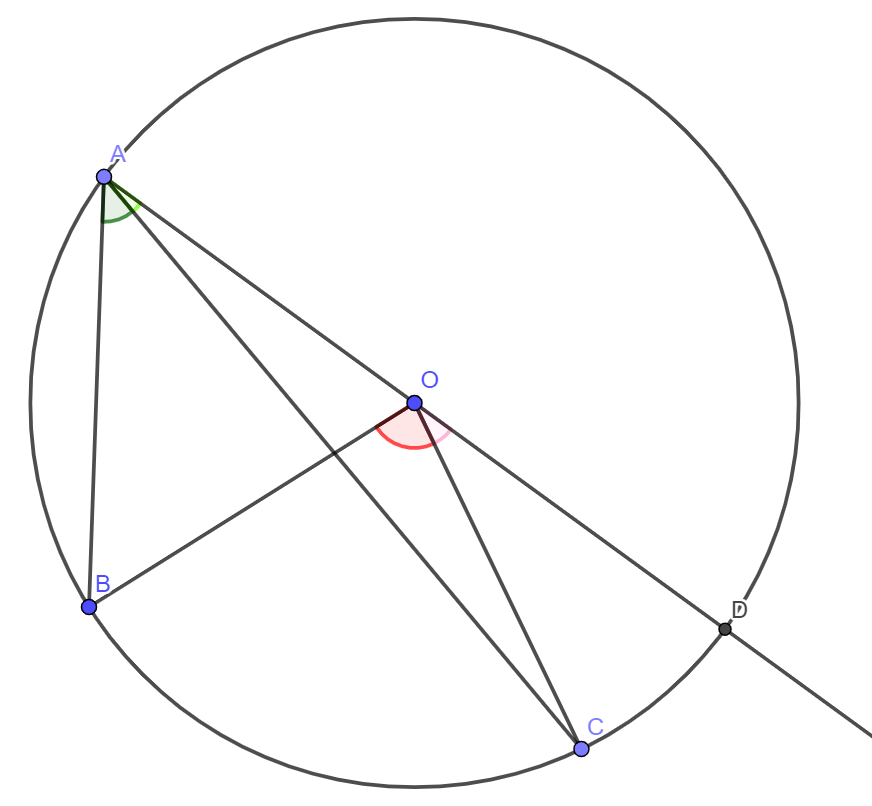
\includegraphics[scale=1]{A-17-PM/A-17-PM-10.png}}\newline
On trace le diamètre $AD$ et on utilise le premier cas :
\[
\widehat{BOC}=\widehat{BOD}-\widehat{COD}=2\widehat{BAD}-2\widehat{CAD}=2\widehat{BAC}.
\]

\end{preuve}

Il convient de noter que la plupart du temps, nous n'aurons pas besoin de l'angle au centre. On utilisera directement le fait que tous les angles inscrits interseptant le même arc sont égaux : on appelera ceci le \emph{théorème de l'angle inscrit}. Il convient également de noter que \emph{tout angle inscrit interseptant le diamètre est droit}.

Il est également intéressant de connaître le cas limite du théorème de l'angle inscrit : le théorème de l'angle tangent. Il vous sera présenté pendant la deuxième séance.

Enfin, notons que le théorème de l'angle au centre et de l'angle inscrit permet de caractériser les quadrilatères insciptibles, et c'est un des outils fondamentaux de la chasse aux angles.

\begin{dfn}
Un polygone est dit \emph{inscriptible} lorsqu'il existe un cercle qui passe par tous ses sommets.
\end{dfn}

Commençons par remarquer qu'un triangle est toujours inscriptible, chose dont on se convainc en démontrant que les trois médiatrices d'un triangle sont concourantes. Pour déterminer si un quadrilatère est insciptible, on dispose du \emph{théorème du quadrilatère inscriptible} :

\begin{thm}
Si un quadrilatère est inscriptible, alors la somme de ses angles opposés vaut $180^\circ$.
\end{thm}
\centering{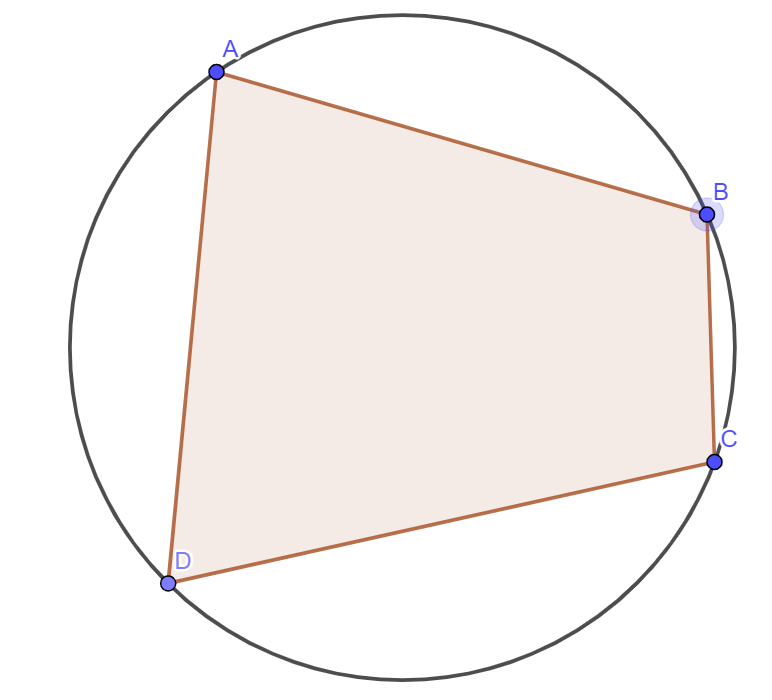
\includegraphics[scale=1]{A-17-PM/A-17-PM-11.png}}\newline

On remarque que si la somme de deux angles opposés d'un quadrilatère vaut $180^\circ$, alors la somme des deux autres angles opposés du quadrilatère vaut aussi $180^\circ$ car la somme des angles d'un quadrilatère vaut $360^\circ$.

\begin{preuve}
Supposons que $ABCD$ est un quadrilatère inscriptible. Montrons que $\widehat{B}+\widehat{D}=180^\circ$.
$\widehat{B}$ et $\widehat{D}$ sont des angles inscrits, donc le premier se mesure comme la moitié de l'angle au centre interseptant l'arc $\stackrel \frown{ADC}$ et le deuxième se mesure comme la moitié de l'angle au centre interseptant l'arc $\stackrel \frown{ABC}$. Comme la somme des deux arcs donne le cercle complet, la somme des deux angles au centre vaut $360^\circ$. Donc, $\widehat{B}+\widehat{D}=180^\circ$.
\end{preuve}

Il sera également très important pour les chasses aux angles d'utiliser les réciproques du théorème des angles inscrits et du théorème du quadrilatère inscriptible. Elles nous permettent de démontrer qu'on a des points cocycliques à partir d'égalités d'angles.

\subsubsection{Exercices sur la chasse aux angles}
\begin{exo}
Soient $C_{1}$ et $C_{2}$ deux cercles ayant deux points d'intersection
$A$ et $B$. Soit $d_{A}$ une droite passant par $A$ et $d_{B}$
une droite passant par $B$. On note $C$ et $E$ les points d'intersection
de $d_{A}$ avec $C_{1}$ et $C_{2}$ respectivement, et on définit
de même $D$ et $F$ comme les points d'intersection de $d_{B}$ avec
$C_{1}$ et $C_{2}$ respectivement. Montrer que les droites $(CD)$
et $(EF)$ sont parallèles.
\end{exo}

\begin{sol}
Il y a plusieurs façons de tracer la figure pour cet exercice, mais la solution est essentiellement la même, peu importe la configuration considérée (quitte à remplacer certains théorèmes de l'angle inscrit par des théorèmes du quadrilatère inscriptible). Nous allons faire notre raisonnement en nous appuyant sur la figure suivante, mais on invite le lecteur à tracer des figures différentes pour se convaincre que le raisonnement est essentiellement le même :
\centering{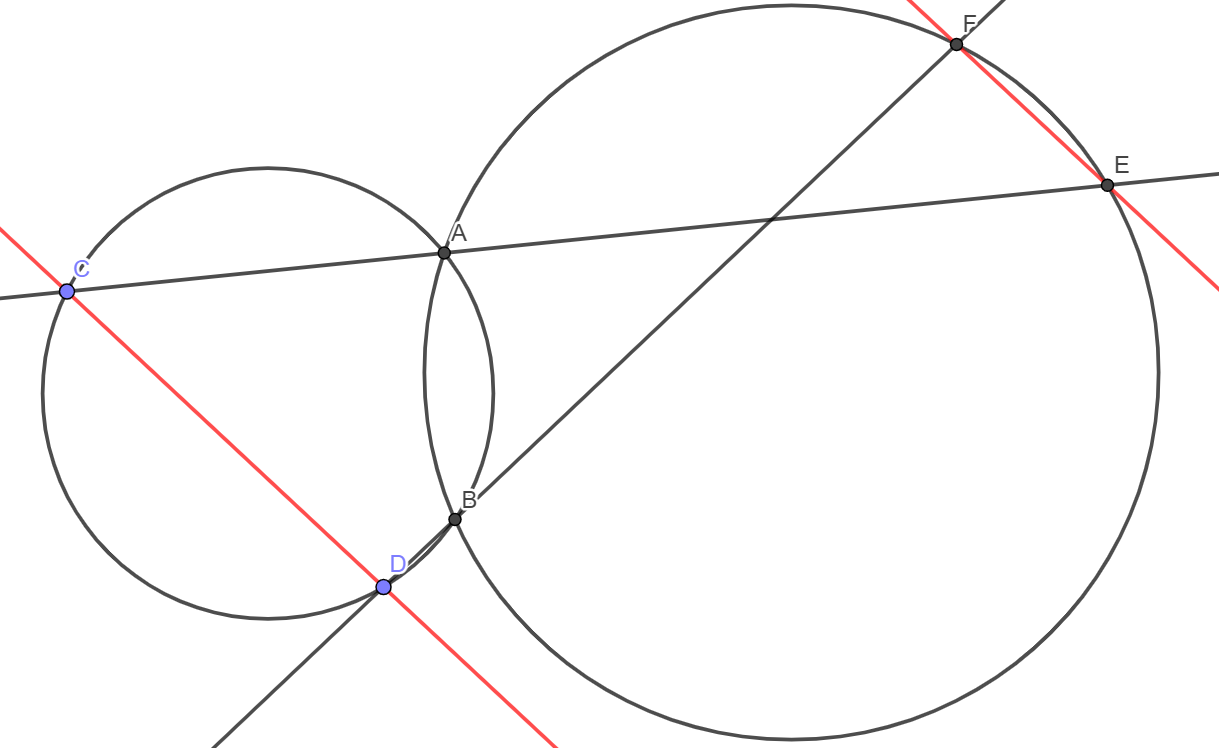
\includegraphics[scale=1]{A-17-PM/A-17-PM-12.png}}\newline
On veut montrer que les droites $(CD)$ et $(EF)$ sont parallèles.

Quand on a deux cercles qui s'intersectent, il est une bonne idée de tracer leur droite d'intersection. On a maintenant assez d'éléments de tracés pour démarrer une chasse aux angles sur la figure.
\centering{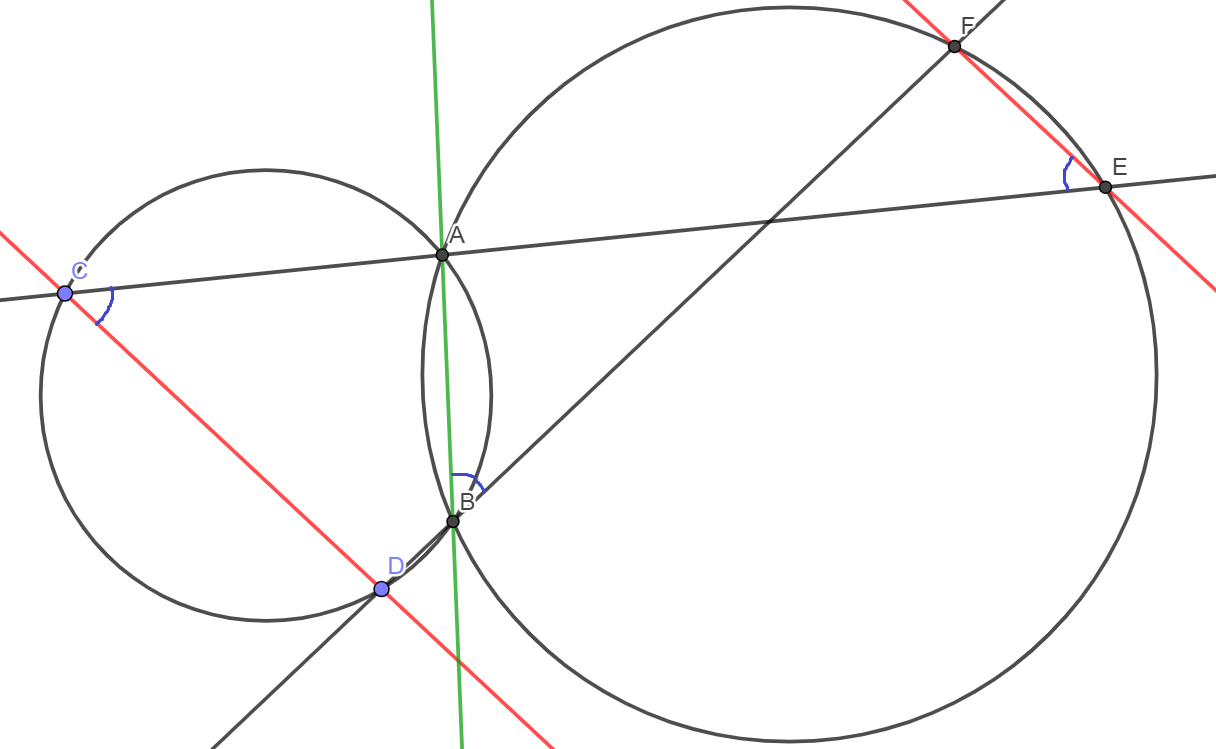
\includegraphics[scale=1]{A-17-PM/A-17-PM-13.png}}\newline
D'après les angles alternes-internes, pour montrer que les droites $(CD)$ et $(EF)$ sont parallèles, il suffit de montrer que l'angle $\widehat{DCA}$ est égal à l'angle $\widehat{AEF}$. Montrons cette égalité d'angles par chasse aux angles.

Puisque le quadrilatère $ABDC$ est inscriptible, on a que les angles $\widehat{DCA}$ et $\widehat{ABD}$ sont supplémentaires. Comme la somme de $\widehat{ABD}$ et $\widehat{ABF}$ donne l'angle plat, on en déduit que les angles $\widehat{DCA}$ et $\widehat{ABF}$ sont égaux. Enfin, d'après le théorème de l'angle inscrit, $\widehat{ABF}=\widehat{AEF}$.

Ainsi, $\widehat{DCA}=\widehat{AEF}$ et c'est ce qu'on voulait.
\end{sol}

\begin{exo}
Soit $ABC$ un triangle, $P$ un point du côté $BC$, $Q$ un point
du côté $CA$ et $R$ un point du côté $AB$. Les cercles circonscrits
à $AQR$ et $BRP$ ont pour second point d'intersection $X$. Montrer
que $X$ est aussi sur le cercle circonscrit à $CPQ$.
\end{exo}

\begin{sol}
On commence bien sûr par tracer une figure et mettre en pointillés le cercle dont nous voulons démontrer l'existence :
\centering{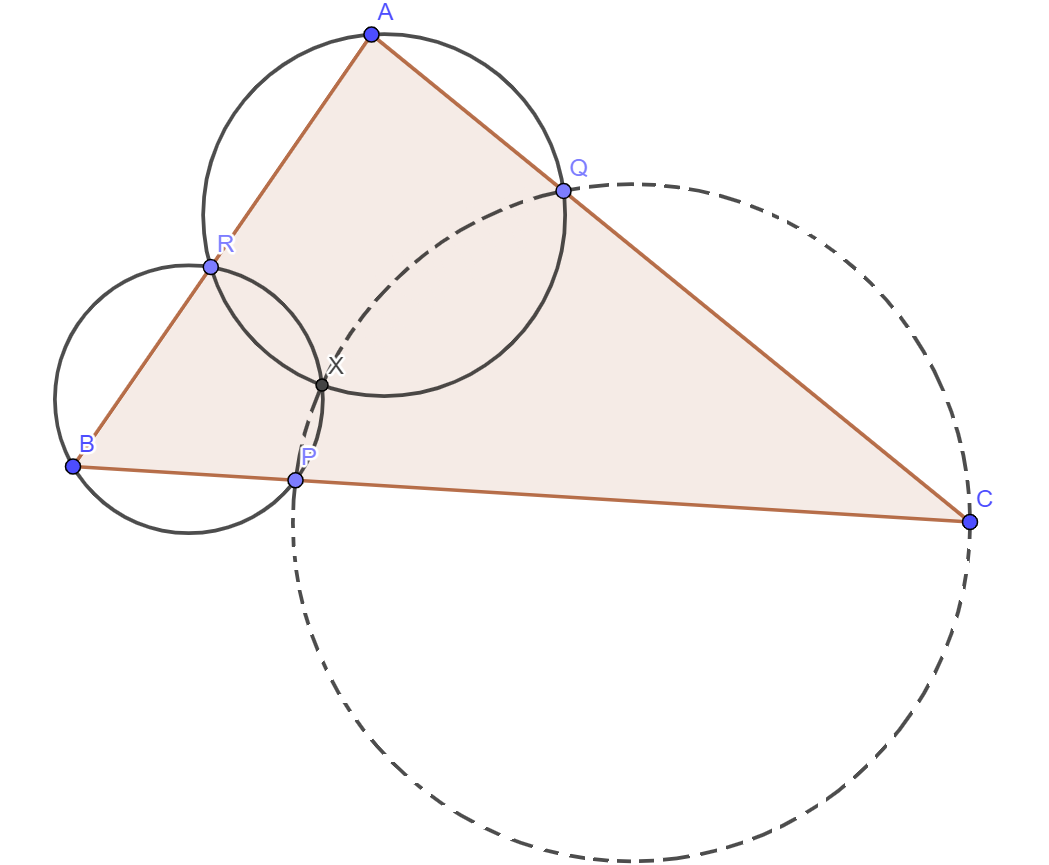
\includegraphics[scale=1]{A-17-PM/A-17-PM-14.png}}\newline
Traçons les droites d'intersection des cercles qui s'intersectent et démarrons une chasse aux angles sur la figure. Deux chasses aux angles différentes ont été proposées par les élèves. Dans tous les cas, notre objectif est de montrer que le quadrilatère $CPXQ$ est inscriptible.

\underline{\textit{Première version :}} Pour y arriver, nous allons montrer que $\widehat{XQC}+\widehat{XPC}=180^\circ$.
\centering{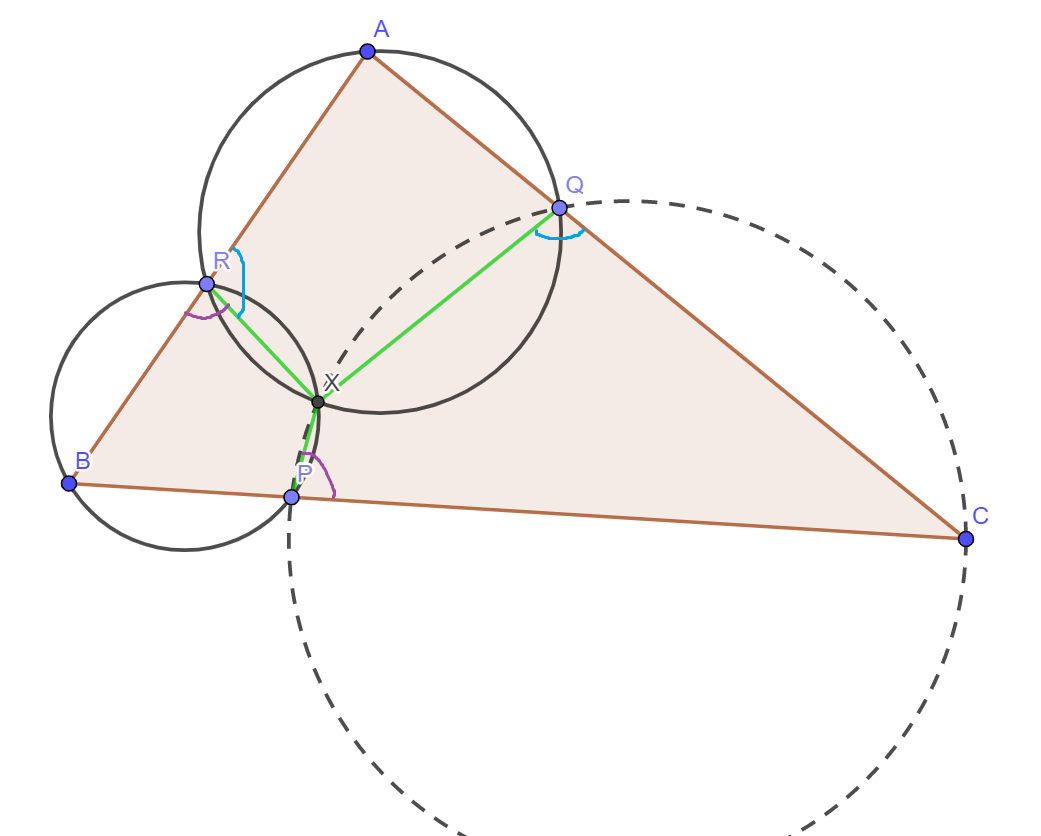
\includegraphics[scale=1]{A-17-PM/A-17-PM-15.png}}\newline
Comme les points $B,P,C$ sont alignés, on a que $\widehat{BPX}+\widehat{XPC}=180^\circ$. Comme le quadrilatère $RXPB$ est inscriptible, on a que $\widehat{BRX}+\widehat{BPX}=180^\circ$.

Donc, $\widehat{XPC}=\widehat{BRX}$.

Par le même raisonnement, $\widehat{XQC}=\widehat{XRA}$.

Or, $\widehat{BRX}+\widehat{XRA}=180^\circ$ car $B,R,A$ sont alignés. Donc, $\widehat{XQC}+\widehat{XPC}=180^\circ$ en découle.

\underline{\textit{Deuxième version :}} Pour y arriver, nous allons montrer que $\widehat{PXQ}+\widehat{QCP}=180^\circ$.
\centering{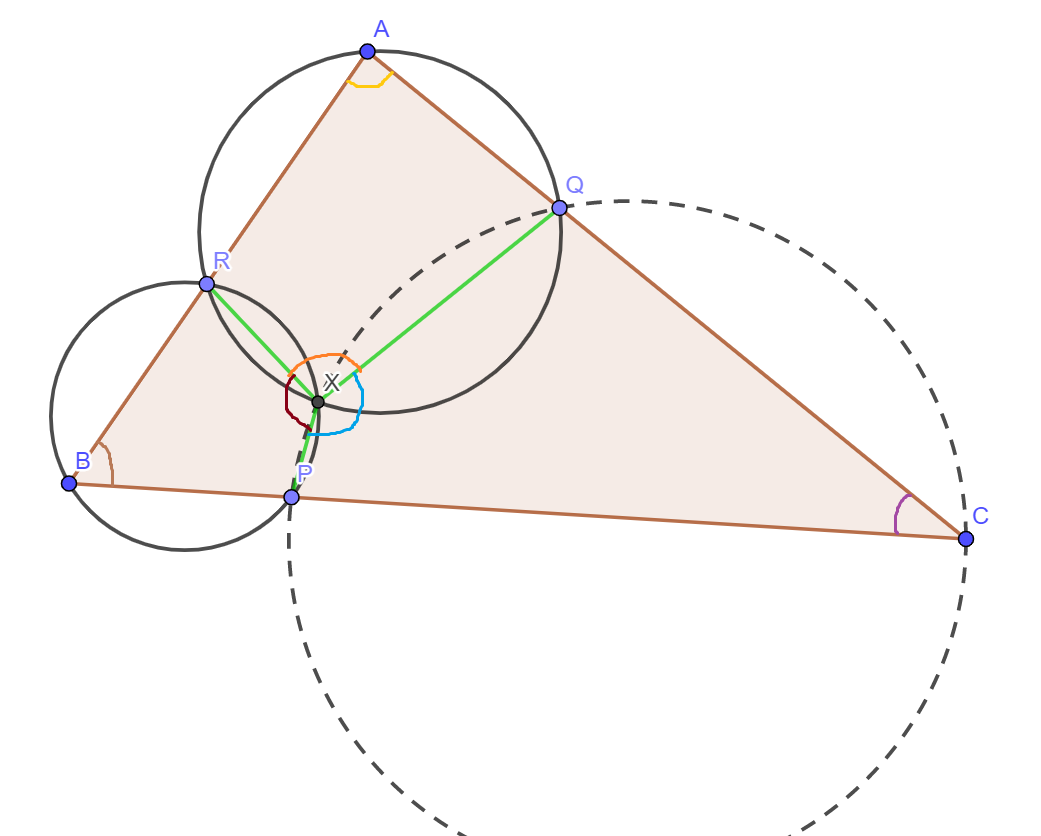
\includegraphics[scale=1]{A-17-PM/A-17-PM-16.png}}\newline
En faisant le tour autour du point $X$, on s'aperçoit que
\[
\widehat{PXQ}+\widehat{QXR}+\widehat{RXP}=360^\circ.
\]
D'après la somme des angles du triangle $ABC$, on a
\[
\widehat{QCP}+\widehat{RAQ}+\widehat{PBR}=180^\circ.
\]
De plus, comme les quadrilatères $XQAR$ et $XRBP$ sont inscriptibles, on a
\[
\widehat{QXR}+\widehat{RAQ}=180^\circ,
\]
et
\[
\widehat{RXP}+\widehat{PBR}=180^\circ.
\]
En mettant toutes ces informations ensemble, on en déduit que
\[
\widehat{PXQ}+\widehat{QCP}=360^\circ-(\widehat{QXR}+\widehat{RXP})+180^\circ-(\widehat{RAQ}+\widehat{PBR})=3 \cdot 180^\circ -(\widehat{QXR}+\widehat{RAQ})-(\widehat{RXP}+\widehat{PBR})=3 \cdot 180^\circ -2 \cdot 180^\circ=180^\circ,
\]
ce qui termine la démonstration.
\end{sol}


\subsubsection{Résumé des outils appris ou révisés pendant la séance}


\begin{itemize}
\item Angles alternes internes, correspondants
\item Somme des angles d'un triangle, d'un polygone
\item Caractérisation d'une médiatrice
\item Dans un triangle, $AB=AC \iff \beta=\gamma$ (critère du triangle isocèle)
\item Les cas d'égalité des triangles
\item Théorème de l'angle au centre et de l'angle inscrit, cas du quadrilatère inscriptible
\end{itemize}